% fig_tr09_comparison.tex — TR-08 vs TR-09 performance comparison bar chart
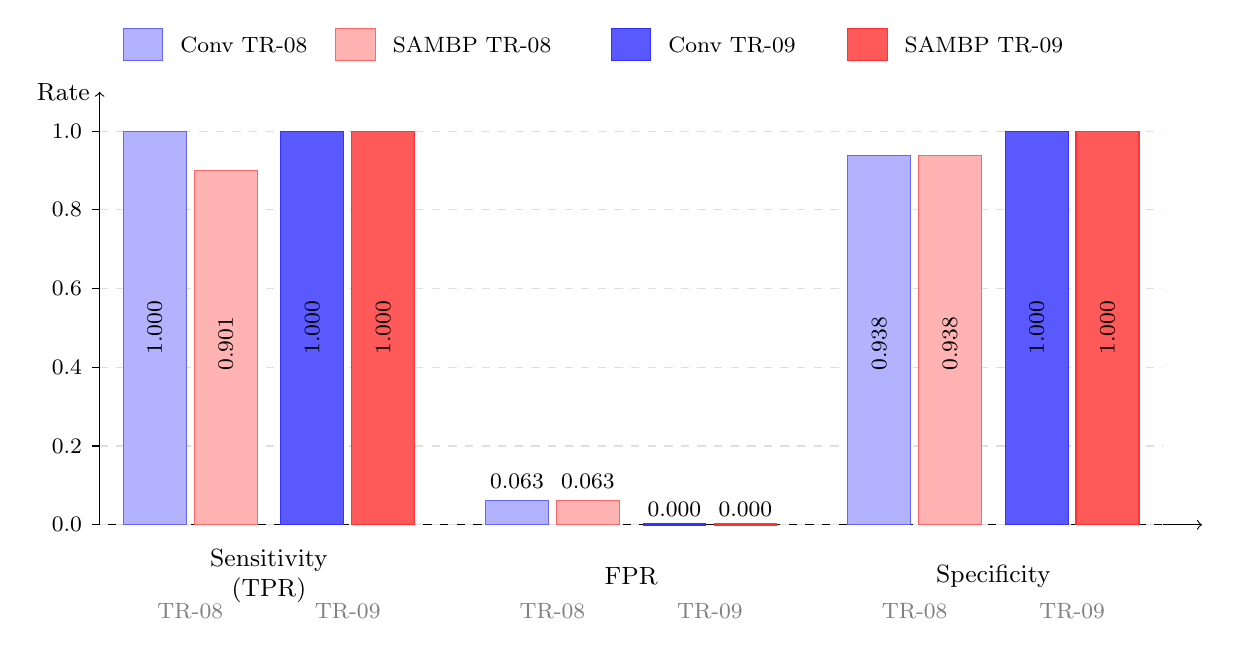
\begin{tikzpicture}

\def\H{5.0}

% Axes
\draw[->] (0,0) -- (0,\H+0.5) node[left,font=\small]{Rate};
\draw[->] (0,0) -- (14.0,0)   node[below,font=\small]{};

% Y-axis
\foreach \y/\val in {0/0.0,1.0/0.2,2.0/0.4,3.0/0.6,4.0/0.8,5.0/1.0}{
    \draw (0,\y) -- (-0.1,\y) node[left,font=\footnotesize]{\val};
    \draw[gray!25,dashed] (0,\y) -- (13.5,\y);
}

% -------- Group 1: Sensitivity --------
%  TR-08 Conv=1.00 / SAMBP=0.901
%  TR-09 Conv=1.00 / SAMBP=1.000

% TR-08 bars (hatched = TR-08)
\fill[blue!30]  (0.3,0) rectangle (1.1,5.0);
\draw[blue!60]  (0.3,0) rectangle (1.1,5.0);
\fill[red!30]   (1.2,0) rectangle (2.0,4.503);
\draw[red!60]   (1.2,0) rectangle (2.0,4.503);

% TR-09 bars (solid = TR-09)
\fill[blue!65]  (2.3,0) rectangle (3.1,5.0);
\draw[blue!80]  (2.3,0) rectangle (3.1,5.0);
\fill[red!65]   (3.2,0) rectangle (4.0,5.0);
\draw[red!80]   (3.2,0) rectangle (4.0,5.0);

\node[font=\footnotesize,rotate=90] at (0.7,2.5)  {1.000};
\node[font=\footnotesize,rotate=90] at (1.6,2.3)  {0.901};
\node[font=\footnotesize,rotate=90] at (2.7,2.5)  {1.000};
\node[font=\footnotesize,rotate=90] at (3.6,2.5)  {1.000};
\node[font=\small,align=center] at (2.15,-0.65) {Sensitivity\\(TPR)};

% -------- Group 2: FPR --------
%  TR-08: both 0.0625
%  TR-09: both 0.000

\fill[blue!30]  (4.9,0) rectangle (5.7,0.3125);
\draw[blue!60]  (4.9,0) rectangle (5.7,0.3125);
\fill[red!30]   (5.8,0) rectangle (6.6,0.3125);
\draw[red!60]   (5.8,0) rectangle (6.6,0.3125);

% TR-09: FPR=0, draw just a line
\draw[blue!80,very thick] (6.9,0) -- (7.7,0);
\draw[red!80,very thick]  (7.8,0) -- (8.6,0);

\node[font=\footnotesize] at (5.3,0.55)  {0.063};
\node[font=\footnotesize] at (6.2,0.55)  {0.063};
\node[font=\footnotesize] at (7.3,0.20)  {0.000};
\node[font=\footnotesize] at (8.2,0.20)  {0.000};
\node[font=\small,align=center] at (6.75,-0.65) {FPR};

% -------- Group 3: Specificity --------
%  TR-08: both 0.9375
%  TR-09: both 1.000

\fill[blue!30]  (9.5,0) rectangle (10.3,4.6875);
\draw[blue!60]  (9.5,0) rectangle (10.3,4.6875);
\fill[red!30]   (10.4,0) rectangle (11.2,4.6875);
\draw[red!60]   (10.4,0) rectangle (11.2,4.6875);

\fill[blue!65]  (11.5,0) rectangle (12.3,5.0);
\draw[blue!80]  (11.5,0) rectangle (12.3,5.0);
\fill[red!65]   (12.4,0) rectangle (13.2,5.0);
\draw[red!80]   (12.4,0) rectangle (13.2,5.0);

\node[font=\footnotesize,rotate=90] at (9.9,2.3)  {0.938};
\node[font=\footnotesize,rotate=90] at (10.8,2.3) {0.938};
\node[font=\footnotesize,rotate=90] at (11.9,2.5) {1.000};
\node[font=\footnotesize,rotate=90] at (12.8,2.5) {1.000};
\node[font=\small,align=center] at (11.35,-0.65) {Specificity};

% ---- Legend ----
\fill[blue!30] (0.3,\H+0.9) rectangle (0.8,\H+1.3); \draw[blue!60] (0.3,\H+0.9) rectangle (0.8,\H+1.3);
\node[right,font=\footnotesize] at (0.9,\H+1.1) {Conv TR-08};

\fill[red!30] (3.0,\H+0.9) rectangle (3.5,\H+1.3); \draw[red!60] (3.0,\H+0.9) rectangle (3.5,\H+1.3);
\node[right,font=\footnotesize] at (3.6,\H+1.1) {SAMBP TR-08};

\fill[blue!65] (6.5,\H+0.9) rectangle (7.0,\H+1.3); \draw[blue!80] (6.5,\H+0.9) rectangle (7.0,\H+1.3);
\node[right,font=\footnotesize] at (7.1,\H+1.1) {Conv TR-09};

\fill[red!65] (9.5,\H+0.9) rectangle (10.0,\H+1.3); \draw[red!80] (9.5,\H+0.9) rectangle (10.0,\H+1.3);
\node[right,font=\footnotesize] at (10.1,\H+1.1) {SAMBP TR-09};

% ---- Report labels ----
\node[font=\footnotesize,gray] at (1.15,-1.1)  {TR-08};
\node[font=\footnotesize,gray] at (3.15,-1.1)  {TR-09};
\node[font=\footnotesize,gray] at (5.75,-1.1)  {TR-08};
\node[font=\footnotesize,gray] at (7.75,-1.1)  {TR-09};
\node[font=\footnotesize,gray] at (10.35,-1.1) {TR-08};
\node[font=\footnotesize,gray] at (12.35,-1.1) {TR-09};

\end{tikzpicture}
